\documentclass[11pt]{article}
\usepackage{multirow}
\usepackage{hyperref}
\usepackage[margin=0.75in, top=1in]{geometry} 
\usepackage{titling} 
\usepackage{fancyhdr}
\usepackage{cancel}
\usepackage{amsmath}
\usepackage{graphicx}
\usepackage{ragged2e}
\usepackage{calc}
\usepackage{here}
\usepackage{siunitx}
\usepackage{float}





\setlength{\droptitle}{-3cm} 
\pagestyle{fancy}
\fancyhf{} 
\lhead{EN.566: Introduction to Computational Materials Modeling 2023 - HW5}
\rhead{Amitabh Roy}

\begin{document}

\section{Problem Description}
The objective of the HW5 is to to numerically study the 2D Ising Model on a n×n lattice with periodic boundary conditions. (N = n$^2$: total number of spins). The report will focus on the ising model, detailed explanation for each section can be found in the later section of the report.

\section{Choose n = 50 and calculate the magnetization M = N⟨s⟩ as a function of temperature (allowing for
enough Monte Carlo sweeps to reach equilibrium) and determine the critical temperature T$_c$. Plot M
vs. T.}

Pseudo-Code:
\begin{enumerate}
    \item \textit{Generate grid for a lattice size \( n \), initialize a \( n \times n \) grid where each site has a spin value of either \( +1 \) or \( -1 \), chosen randomly with 50\% probability.}
    \item \textit{For a given temperature and for a selected number of Monte Carlo sweeps, select any random site, flip the energy, and then accept the flip if the change in energy \( \Delta E < 0 \) or probability(generated using random numbers) \( < \exp\left(-\frac{\Delta E}{k_B T}\right) \).\cite{ref1}\cite{ref2} \\
NOTE: Use 'numba' python module for just-in-time compilation \cite{ref3}}
    \item \textit{Once the Monte Carlo sweep is complete, calculate the average energy, average magnetization, and specific heat for the system, and save the data into some data structures.}
    \item \textit{Change the temperature and repeat step 2.}
    \item \textit{Plot the respective plots.}
\end{enumerate}

From \autoref{fig:1} to \autoref{fig:16}, the heat maps corresponds to the spin configurations at different time steps selected between T = 1.00 to 5.00 (1/K$_B$). Till T = 3.07 (1/K$_B$), the absolute average magnetisation is close to 1 but as soon as the temperature reaches the 'T$_c$' we see a sudden flip in magnetisation and by taking the derivative of the Energy Vs T and Mangnetisation Vs T we can find the temperature at which there was a sudden change in the system's orientation. In \autoref{fig:17} and \autoref{fig:18}, the T$_c$' is found by taking the derivative and values were T$_c$ = 3.48 (1/K$_B$) \& T$_c$ = 3.34 (1/K$_B$) respectively. Similarly the T$_c$ was found from the specific heat plot also by using the 'scipy' library to find the peak, the calculated T$_c$ = 3.48 (1/K$_B$). The accuracy of the calculation can be improved by taking more number of points and taking monte-carlo steps more than $10^6$(For this study due to the computational limitation the monte-carlo steps = $10^6$ ).

\begin{figure}[H]
    \centering
    \begin{minipage}{0.32\textwidth}
        \centering
        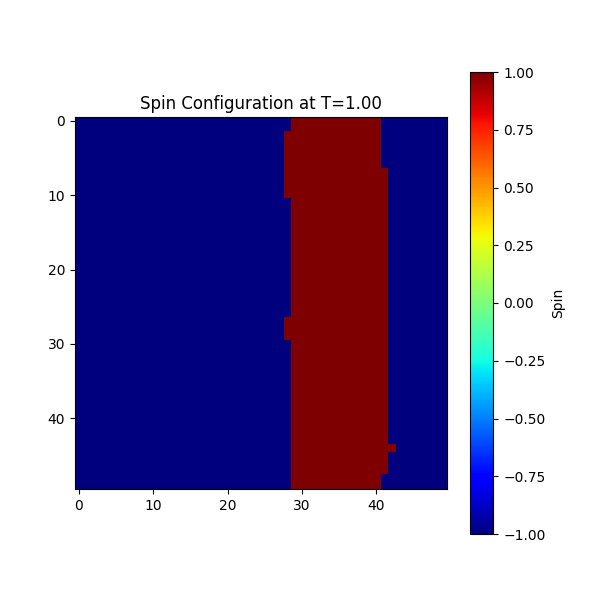
\includegraphics[width=\textwidth]{Spin_Configuration_at_T=1.00.png}
        \caption{Spin Configuration at T = 1.00 (1/K$_B$)}
        \label{fig:1}
    \end{minipage}\hfill
    \begin{minipage}{0.32\textwidth}
        \centering
        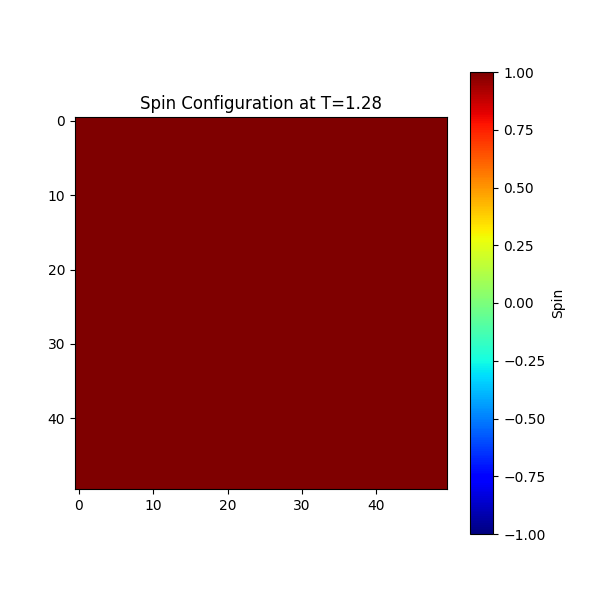
\includegraphics[width=\textwidth]{Spin_Configuration_at_T=1.28.png}
        \caption{Spin Configuration at T = 1.28 (1/K$_B$)}
        \label{fig:2}
    \end{minipage}
    \centering
    \begin{minipage}{0.32\textwidth}
        \centering
        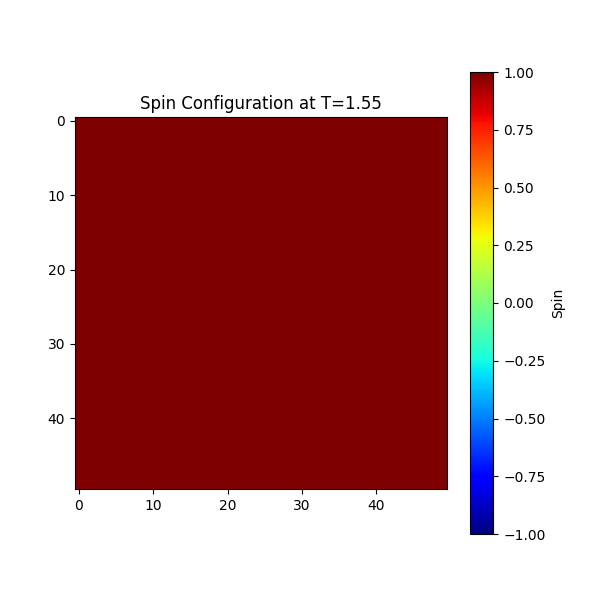
\includegraphics[width=\textwidth]{Spin_Configuration_at_T=1.55.png}
        \caption{Spin Configuration at T = 1.55 (1/K$_B$)}
        \label{fig:3}
    \end{minipage}\hfill
\end{figure}

\begin{figure}[H]
    \begin{minipage}{0.32\textwidth}
        \centering
        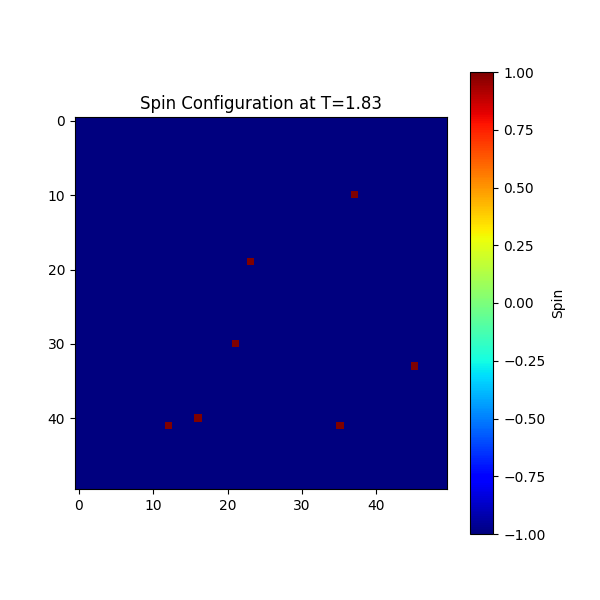
\includegraphics[width=\textwidth]{Spin_Configuration_at_T=1.83.png}
        \caption{Spin Configuration at T = 1.83 (1/K$_B$)}
        \label{fig:4}
    \end{minipage}
    \begin{minipage}{0.32\textwidth}
        \centering
        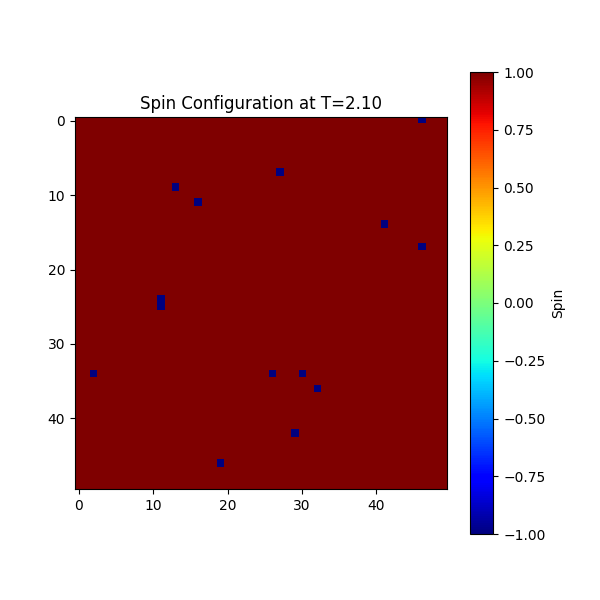
\includegraphics[width=\textwidth]{Spin_Configuration_at_T=2.10.png}
        \caption{Spin Configuration at T = 2.1 (1/K$_B$)}
        \label{fig:5}
    \end{minipage}\hfill
    \begin{minipage}{0.32\textwidth}
        \centering
        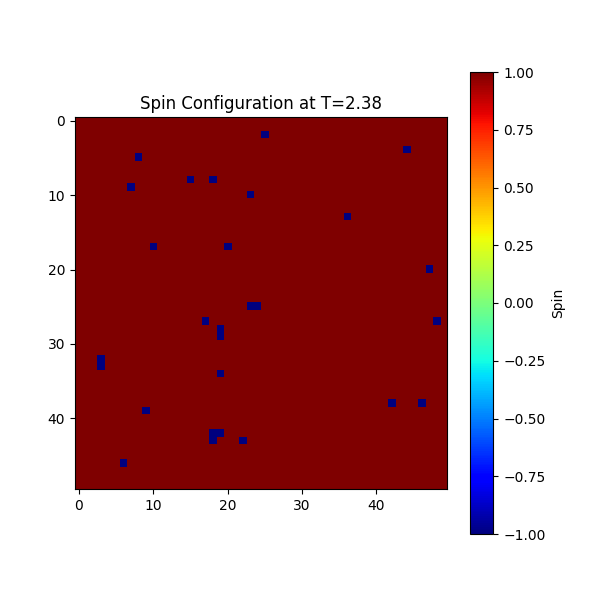
\includegraphics[width=\textwidth]{Spin_Configuration_at_T=2.38.png}
        \caption{Spin Configuration at T = 2.38 (1/K$_B$)}
        \label{fig:6}
    \end{minipage}
\end{figure}

\begin{figure}[H]
    \centering
    \begin{minipage}{0.32\textwidth}
        \centering
        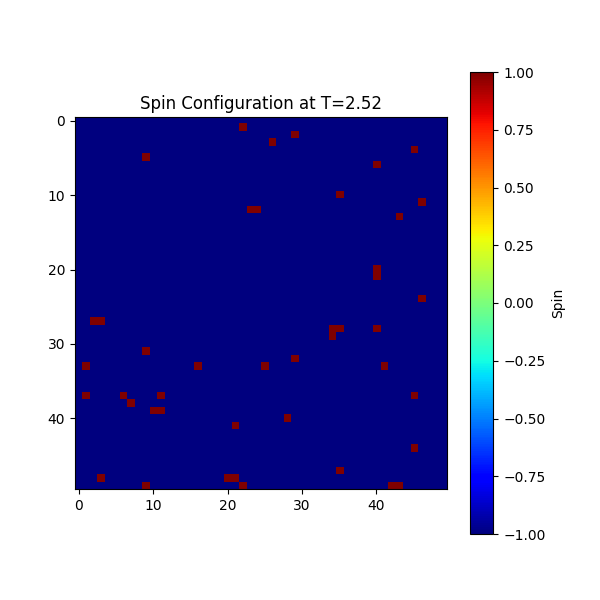
\includegraphics[width=\textwidth]{Spin_Configuration_at_T=2.52.png}
        \caption{Spin Configuration at T = 2.52 (1/K$_B$)}
        \label{fig:7}
    \end{minipage}\hfill
    \begin{minipage}{0.32\textwidth}
        \centering
        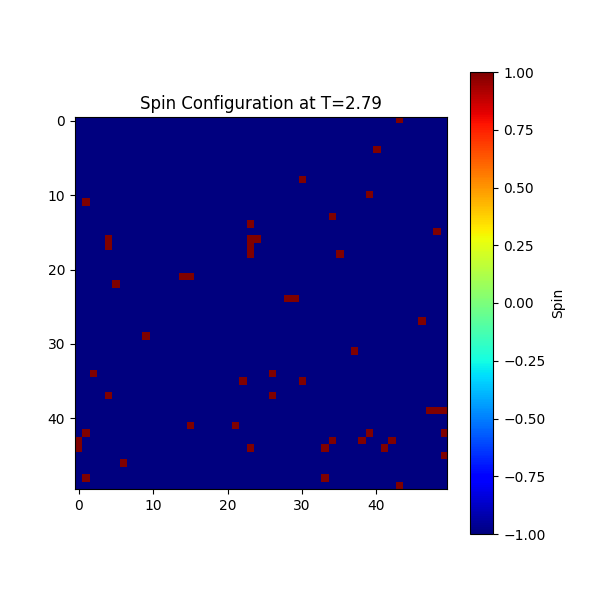
\includegraphics[width=\textwidth]{Spin_Configuration_at_T=2.79.png}
        \caption{Spin Configuration at T = 2.79 (1/K$_B$)}
        \label{fig:8}
    \end{minipage}
        \begin{minipage}{0.32\textwidth}
        \centering
        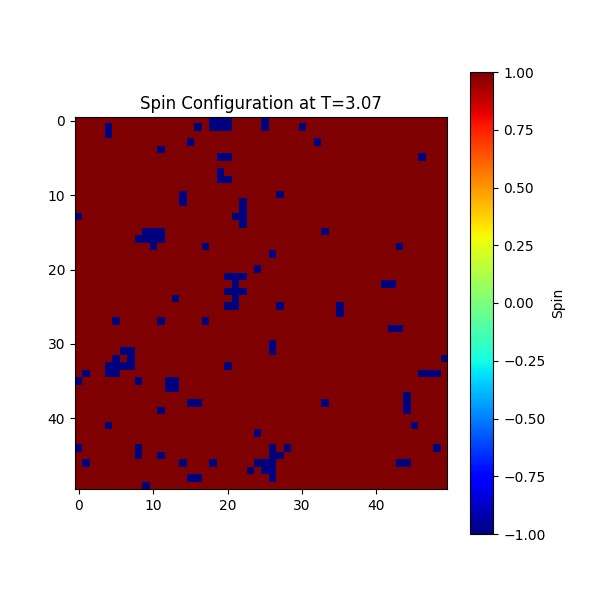
\includegraphics[width=\textwidth]{Spin_Configuration_at_T=3.07.png}
        \caption{Spin Configuration at T = 3.07 (1/K$_B$)}
        \label{fig:9}
    \end{minipage}\hfill
\end{figure}


\begin{figure}[H]
    \centering
    \begin{minipage}{0.32\textwidth}
        \centering
        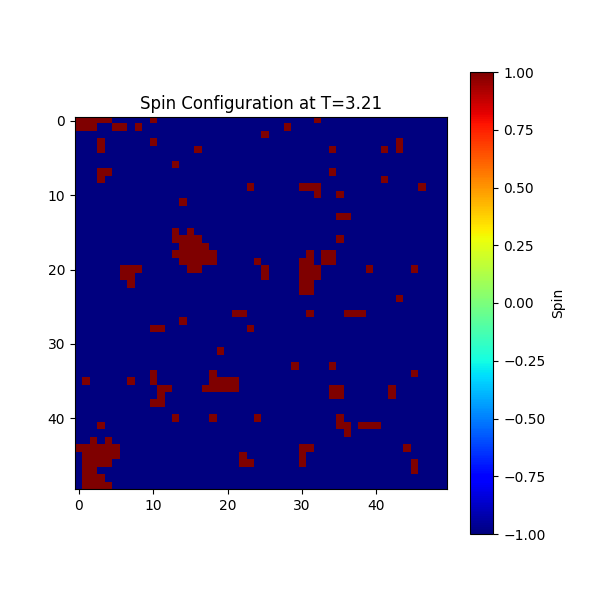
\includegraphics[width=\textwidth]{Spin_Configuration_at_T=3.21.png}
        \caption{Spin Configuration at T = 3.21 (1/K$_B$)}
        \label{fig:10}
    \end{minipage}
    \begin{minipage}{0.32\textwidth}
        \centering
        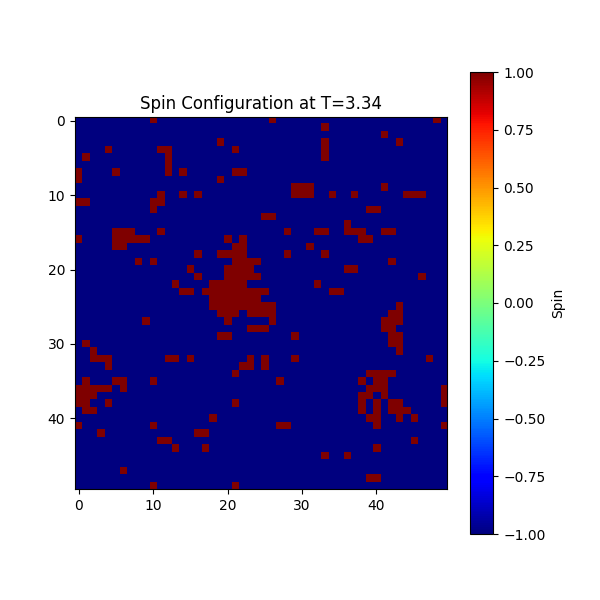
\includegraphics[width=\textwidth]{Spin_Configuration_at_T=3.34.png}
        \caption{Spin Configuration at T = 3.34 (1/K$_B$)}
        \label{fig:11}
    \end{minipage}\hfill
    \begin{minipage}{0.32\textwidth}
        \centering
        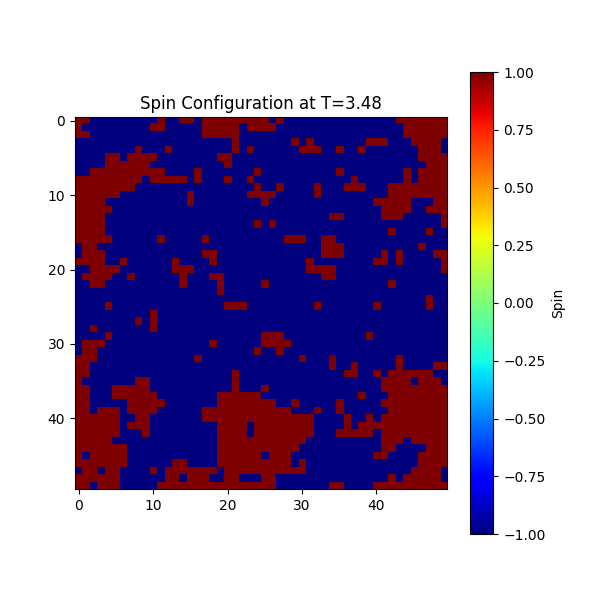
\includegraphics[width=\textwidth]{Spin_Configuration_at_T=3.48.png}
        \caption{Spin Configuration at T = 3.48 (1/K$_B$)}
        \label{fig:12}
    \end{minipage}
\end{figure}

\begin{figure}[H]
    \centering
    \begin{minipage}{0.32\textwidth}
        \centering
        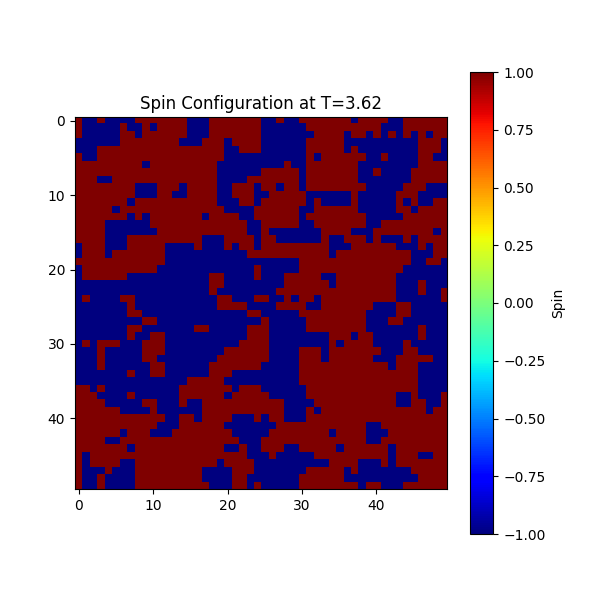
\includegraphics[width=\textwidth]{Spin_Configuration_at_T=3.62.png}
        \caption{Spin Configuration at T = 3.62 (1/K$_B$)}
        \label{fig:13}
    \end{minipage}\hfill
    \begin{minipage}{0.32\textwidth}
        \centering
        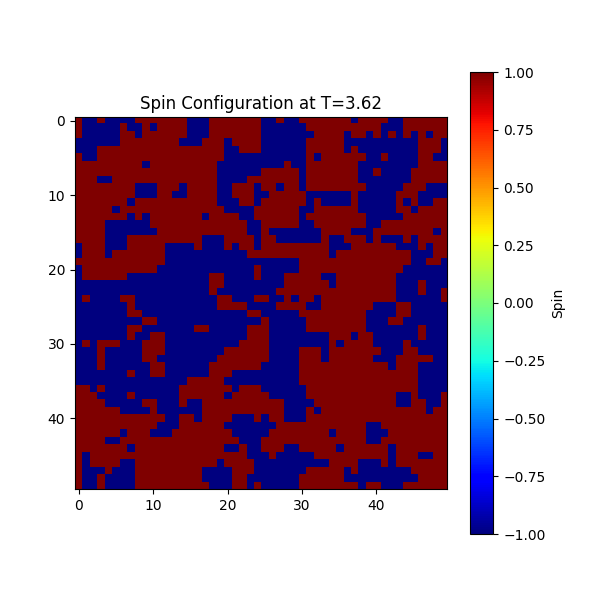
\includegraphics[width=\textwidth]{Spin_Configuration_at_T=3.62.png}
        \caption{Spin Configuration at T = 3.62 (1/K$_B$)}
        \label{fig:14}
    \end{minipage}
    \begin{minipage}{0.32\textwidth}
        \centering
        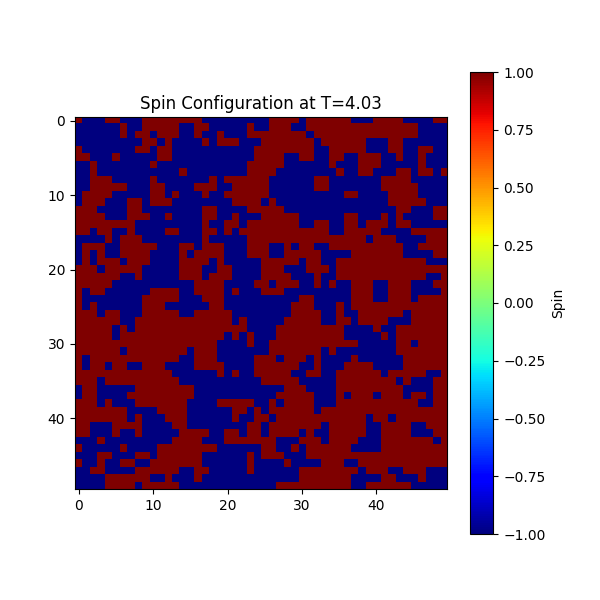
\includegraphics[width=\textwidth]{Spin_Configuration_at_T=4.03.png}
        \caption{Spin Configuration at T = 4.03 (1/K$_B$)}
        \label{fig:15}
    \end{minipage}\hfill
\end{figure}

\begin{figure}[H]
    \centering
    \begin{minipage}{0.32\textwidth}
        \centering
        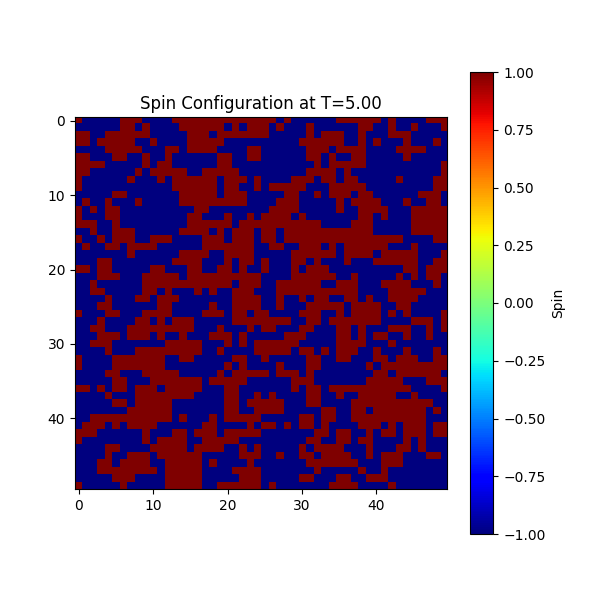
\includegraphics[width=\textwidth]{Spin_Configuration_at_T=5.00.png}
        \caption{Spin Configuration at T = 5.00 (1/K$_B$)}
        \label{fig:16}
    \end{minipage}
\end{figure}

\begin{figure}[H]
    \centering
    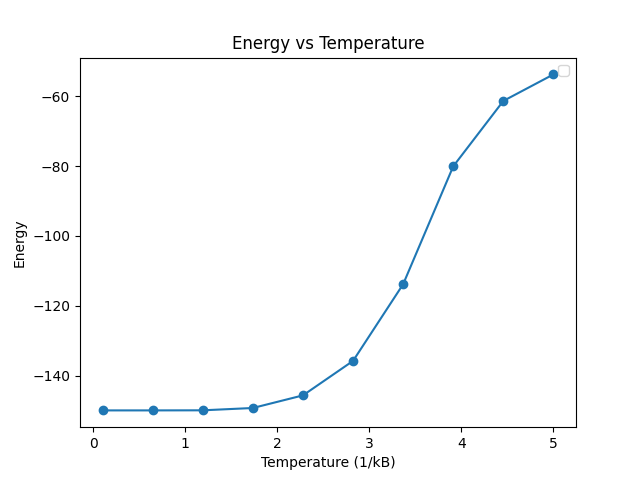
\includegraphics[width=0.48\textwidth, keepaspectratio]{Energy_vs_Temperature.png}
    \caption{Energy Vs Temperature}
    \label{fig:17}
\end{figure}

\begin{figure}[H]
    \centering
    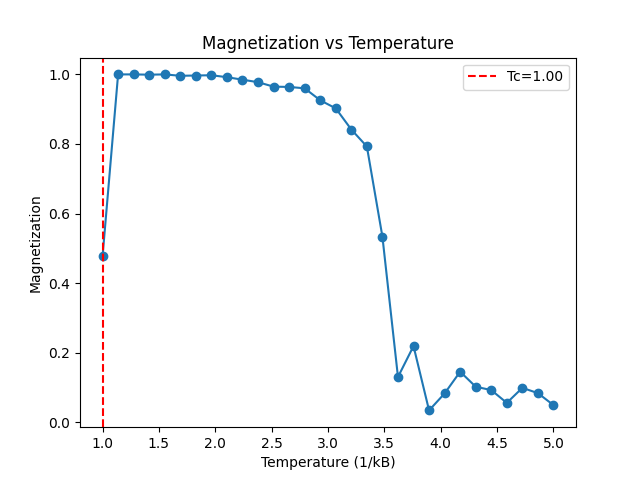
\includegraphics[width=0.48\textwidth, keepaspectratio]{Magnetization_vs_Temperature.png}
    \caption{Magnetization Vs Temperature}
    \label{fig:18}
\end{figure}

\begin{figure}[H]
    \centering
    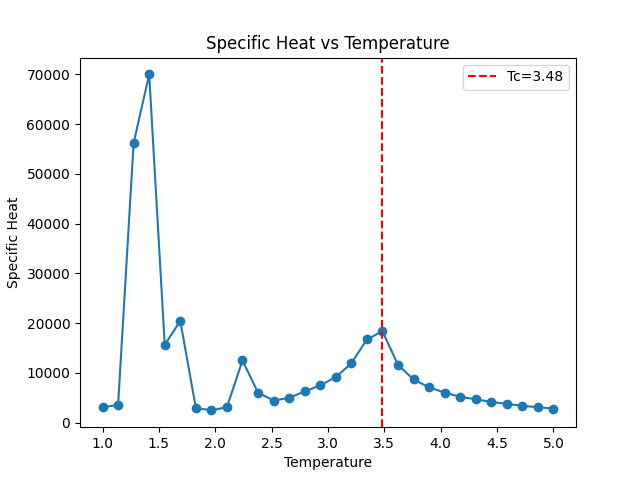
\includegraphics[width=0.48\textwidth, keepaspectratio]{Specific_Heat_vs_Temperature.png}
    \caption{Specific Heat Vs Temperature}
    \label{fig:19}
\end{figure}


\section{Calculate the specific heat per spin C/N for 10 different lattice sizes, n = 5, 10, 20, 30, 40, 50, 75, 100, 200, 500, using the fluctuation-dissipation theorem C = ($\Delta$E)2/(k$_B$T$^2$), and verify the approximate finite-size scaling relation C$_{max}$/N $\sim$ log(n). (Hint: Make sure to use sufficient temperature resolution when determining the maximum in C/N as you increase n. The relation may yield better
results for the smaller values of n). Show figures for C(T) for a few sample cases as well as C$_{max}$/N vs. n.}

Pseudo-Code:
\begin{enumerate}
    \item \textit{Generate a list of all given lattice}
    \item \textit{For a given lattice size repeat all the steps mentioned in section 2}
    \item \textit{Change the lattice size and repeat step 2}
    \item \textit{Plot respective plots}
\end{enumerate}

\autoref{fig:20}, is should be a linear relationship between C$_{max}$/N and log(n), using this relation we can state that C$_{max}$/N $\sim$ log(n).But dur to the computational constraints we did not got the proper stabilized system for larger grid sizes. \autoref{fig:21} to \autoref{fig:30}, shows specific heat vs temp plot for different lattice sizes mentioned in the question.

\begin{figure}[H]
    \centering
    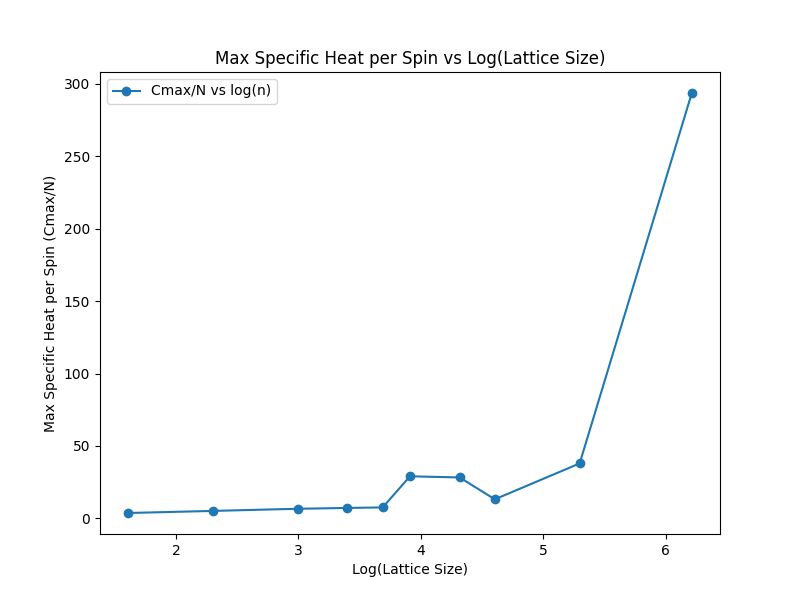
\includegraphics[width=0.48\textwidth, keepaspectratio]{Max_Specific_Heat_per_Spin_vs_Log_Lattice_Size.png}
    \caption{C$_{max}$/N Vs log(n)}
    \label{fig:20}
\end{figure}


\begin{figure}[H]
    \centering
    % Left plot
    \begin{minipage}{0.48\textwidth}
        \centering
        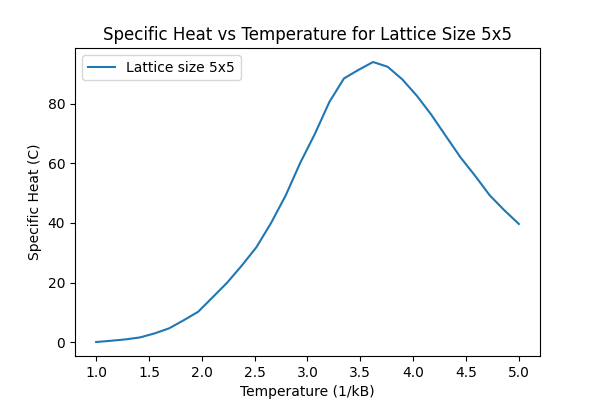
\includegraphics[width=\textwidth]{Specific_Heat_vs_Temperature_n5.png}
        \caption{Specific Heat Vs Temperature; n = 5}
        \label{fig:21}
    \end{minipage}\hfill % Fill space between the two minipages
    % Right plot
    \begin{minipage}{0.48\textwidth}
        \centering
        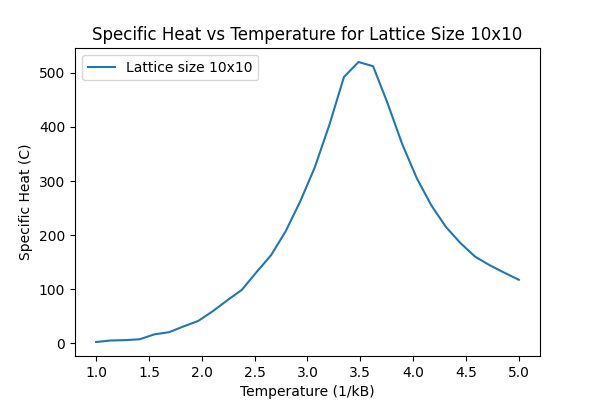
\includegraphics[width=\textwidth]{Specific_Heat_vs_Temperature_n10.png}
        \caption{Specific Heat Vs Temperature; n = 10}
        \label{fig:22}
    \end{minipage}
\end{figure}

\begin{figure}[H]
    \centering
    % Left plot
    \begin{minipage}{0.48\textwidth}
        \centering
        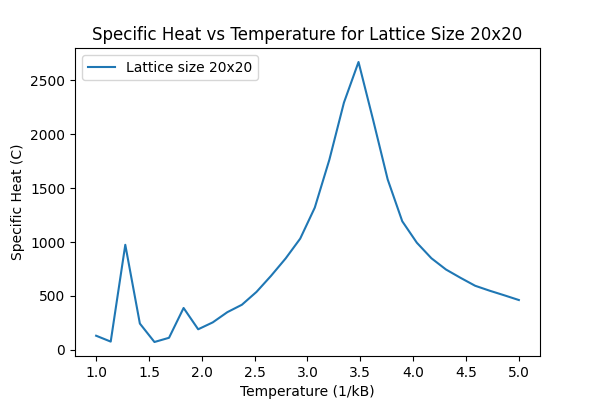
\includegraphics[width=\textwidth]{Specific_Heat_vs_Temperature_n20.png}
        \caption{Specific Heat Vs Temperature; n = 20}
        \label{fig:23}
    \end{minipage}\hfill % Fill space between the two minipages
    % Right plot
    \begin{minipage}{0.48\textwidth}
        \centering
        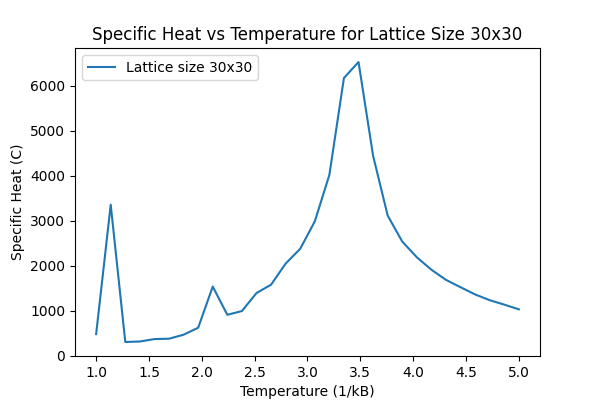
\includegraphics[width=\textwidth]{Specific_Heat_vs_Temperature_n30.png}
        \caption{Specific Heat Vs Temperature; n = 30}
        \label{fig:24}
    \end{minipage}
\end{figure}

\begin{figure}[H]
    \centering
    % Left plot
    \begin{minipage}{0.48\textwidth}
        \centering
        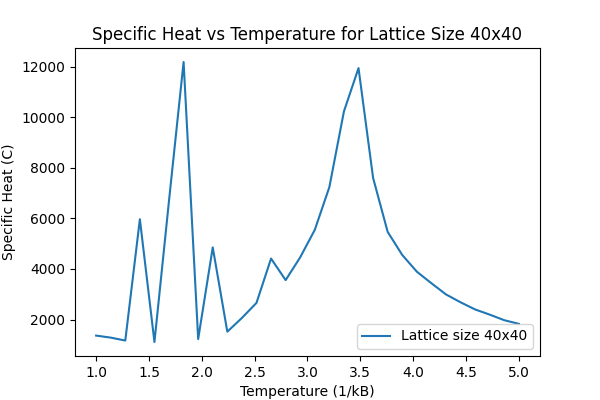
\includegraphics[width=\textwidth]{Specific_Heat_vs_Temperature_n40.png}
        \caption{Specific Heat Vs Temperature; n = 40}
        \label{fig:25}
    \end{minipage}\hfill % Fill space between the two minipages
    % Right plot
    \begin{minipage}{0.48\textwidth}
        \centering
        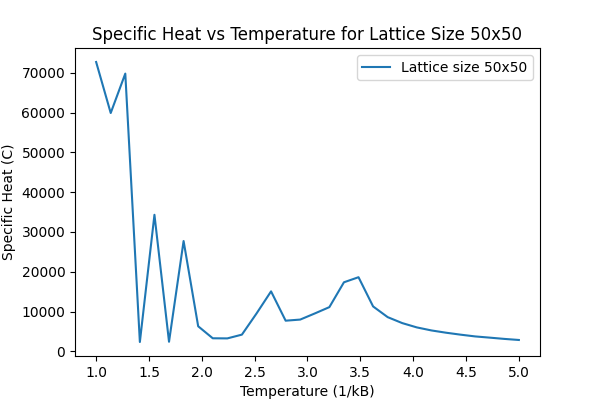
\includegraphics[width=\textwidth]{Specific_Heat_vs_Temperature_n50.png}
        \caption{Specific Heat Vs Temperature; n = 50}
        \label{fig:26}
    \end{minipage}
\end{figure}

\begin{figure}[H]
    \centering
    % Left plot
    \begin{minipage}{0.48\textwidth}
        \centering
        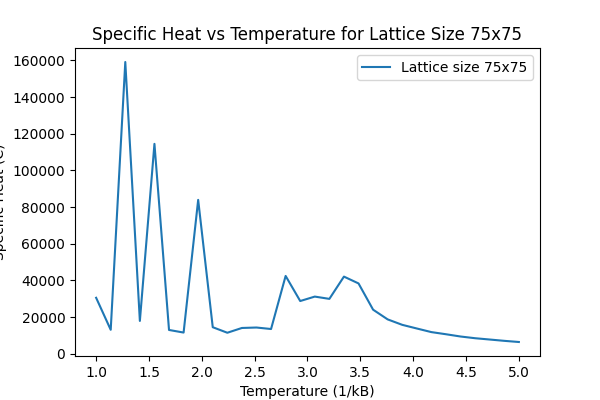
\includegraphics[width=\textwidth]{Specific_Heat_vs_Temperature_n75.png}
        \caption{Specific Heat Vs Temperature; n = 75}
        \label{fig:27}
    \end{minipage}\hfill % Fill space between the two minipages
    % Right plot
    \begin{minipage}{0.48\textwidth}
        \centering
        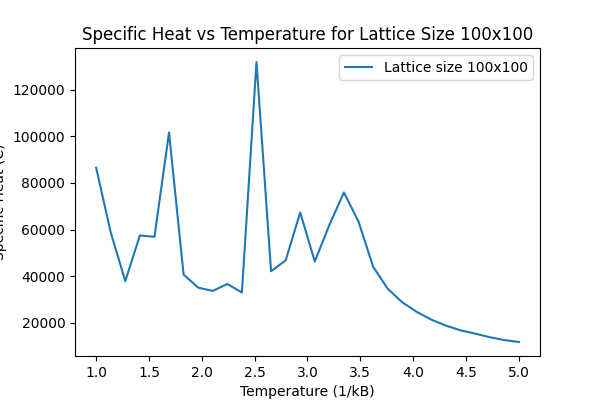
\includegraphics[width=\textwidth]{Specific_Heat_vs_Temperature_n100.png}
        \caption{Specific Heat Vs Temperature; n = 100}
        \label{fig:28}
    \end{minipage}
\end{figure}

\begin{figure}[H]
    \centering
    % Left plot
    \begin{minipage}{0.48\textwidth}
        \centering
        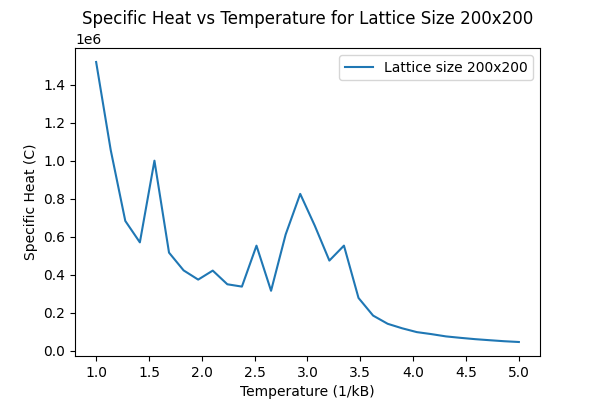
\includegraphics[width=\textwidth]{Specific_Heat_vs_Temperature_n200.png}
        \caption{Specific Heat Vs Temperature; n = 200}
        \label{fig:29}
    \end{minipage}\hfill % Fill space between the two minipages
    % Right plot
    \begin{minipage}{0.48\textwidth}
        \centering
        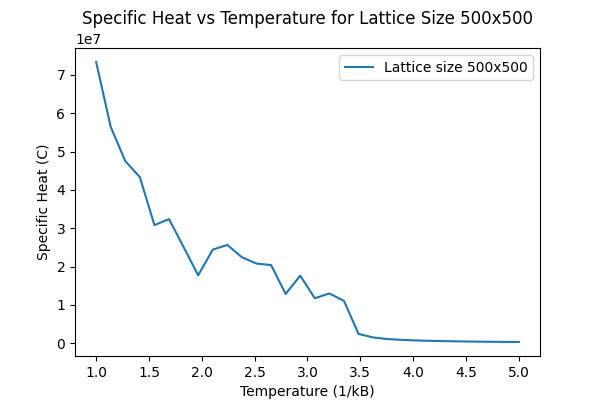
\includegraphics[width=\textwidth]{Specific_Heat_vs_Temperature_n500.png}
        \caption{Specific Heat Vs Temperature; n = 500}
        \label{fig:30}
    \end{minipage}
\end{figure}

\begin{figure}[H]
    \centering
    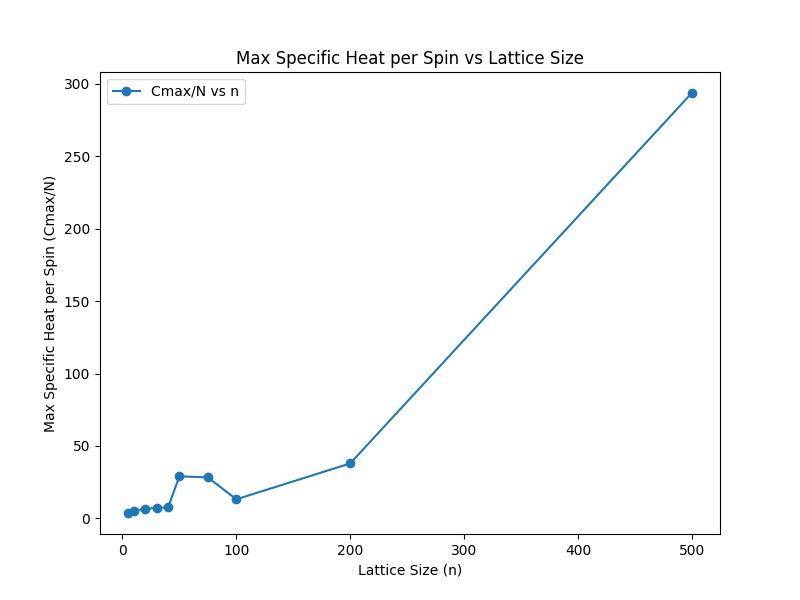
\includegraphics[width=0.48\textwidth, keepaspectratio]{Max_Specific_Heat_per_Spin_vs_Lattice_Size.png}
    \caption{C$_{max}$/N Vs n)}
    \label{fig:31}
\end{figure}


\section{Conclusion}
\begin{enumerate}
  \item From magnetisation vs T, the T$_c$ was calculated to be  3.34 (1/K$_B$
  \item We can see the trend that with increase in lattice size the value for specific heat is also increasing,but to get the accurate data we have to run the simulations for much longer steps
\end{enumerate}

\begin{thebibliography}{}
\bibitem{ref1} T. Theuns. Lecture Notes on Computational Astrophysics. Durham University. Available at: \url{http://star-www.dur.ac.uk/~tt/MSc/Lecture8.pdf}
\bibitem{ref2} B.D. Hammel. The Ising Model. Available at: \url{http://www.bdhammel.com/ising-model/}.
\bibitem{ref3} YouTube Video: The Ising Model in Python: Statistical Mechanics and Permanent Magnets. Available at: \url{https://www.youtube.com/watch?v=K--1hlv9yv0}

\end{thebibliography}

\end{document}